\documentclass{article}
\usepackage{color}
\usepackage{xcolor}
\usepackage{listings}
\usepackage{caption}
\usepackage{xparse}
\usepackage{amsmath}
\usepackage{mathtools}
\usepackage{graphicx}
\usepackage{placeins}
\usepackage{fancyvrb}
\usepackage[OT4]{polski}
\usepackage[utf8]{inputenc}
\usepackage[a4paper]{geometry}
\newgeometry{left=3cm,right=3cm}

\title{Sprawozdanie z realizacji laboratorium z wprowadzenie do przetwarzania obrazów }
\author{Artur Szajdecki}
\date{23 Stycznia 2017}
\begin{document}
\maketitle
To jest sprawozdanie prezentujące operacje na obrazkach dzięki programowi Imgus.

\FloatBarrier
\section{Wstęp}
Program został napisany w C++ i służy do obróbki obrazów PNG, dany program może wczytać obrazy 24-bitowych z kanałami RGB, 8-bitowych o odcieniem szarości i 1-bitowych binarne. Zazwyczaj operacja jest przeprowadzana na jednym obrazie, ale jest możliwość wykonania operacji na dwóch obrazach.
Uwaga! Program nie wczytuje obrazów barwnych z dodatkowym kanałem alpha jak i obrazów o odcieniu szarości z dodatkowym kanałem alpha.

\FloatBarrier
\section{Instrukcja Obsługi}
\begin{figure}[!htb]
\centering
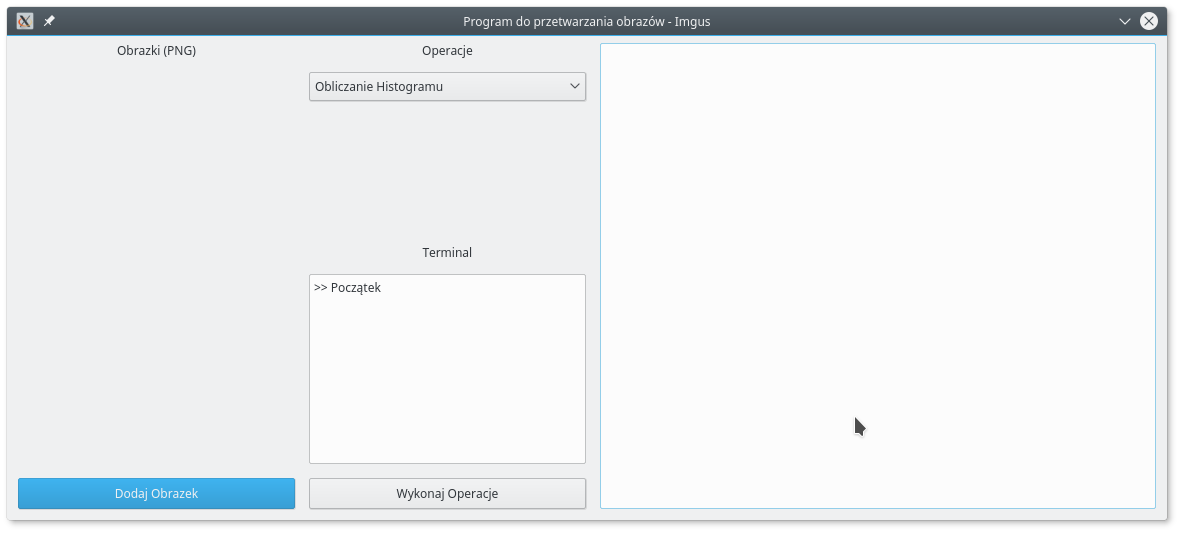
\includegraphics[scale=0.4]{img/software.png} 
\caption{Tak wygląda program Imgus.}
\label{fig:verticalcell}
\end{figure}
Pierwsza kolumna pokazuje wczytane obrazki i można dodać następne obrazy za pomocą przycisku na dole. Druga kolumna pokazuje listę rozwijaną z dostępnymi operacjami które można przeprowadzić na obrazie/kach plus listę parametrów które potrzeba na operacje (Na Rysunku 1 i 2 nie widać listy parametrów bo na obliczanie histogramu nie trzeba parametrów) następnie mamy terminal w którym wyświetlają się komunikaty o błędach czy o pomyślnych przeprowadzonej operacji a pod terminalem mamy przycisk dzięki któremu możemy przeprowadzić operacje. Trzecia kolumna prezentuje wyświetlany obrazek przed/po operacją.\\

Przy każdym obrazku jest informacja o nazwie, wysokości, szerokości i typie (Rysunek 2), typ może być Binarny odpowiadający 1-bit grayscale, Szary odpowiadający 8-bit grayscale i Barwny odpowiadający 24-bit truecolor i po tych informacjach mamy przycisk Skasuj który usuwa obrazek z listy i daje pierwszeństwo obrazkowi drugiemu.\\
Ważną rzeczą jest to że po kliknięciu 'Wykonaj Operacje' wykona się operacja dla pierwszego obrazka z listy i po operacji obrazek przetworzony się zapisze w folderze /img (konieczność jest żeby folder istniał tam gdzie program wykonalny) następnie obrazek zmodyfikowany się wyświetli w kolumnie trzeciej. Również ważna rzeczą jest operacja na dwóch obrazach. Jeśli chcemy przeprowadzić operacje na dwóch obrazach to wczytany pierwszy obrazek i drugi w kolejce muszą być jednolite to znaczy muszą mieć wysokość, szerokość i typ taki sam!\\

Przy operacja która ma możliwość przeprowadzenie czynności na dwóch obrazkach ta operacja może wymusić od programu czynności na dwóch obrazkach chociaż nie chcieliśmy tego (chcieliśmy na przykład przeprowadzić operacje na stałej) w tym przypadku trzeba usunąć każdy obrazek przed pierwszym obrazkiem z listy w pierwszej kolumnie. To jest mała niedoskonałość tego programu.

\begin{figure}[!htb]
\centering
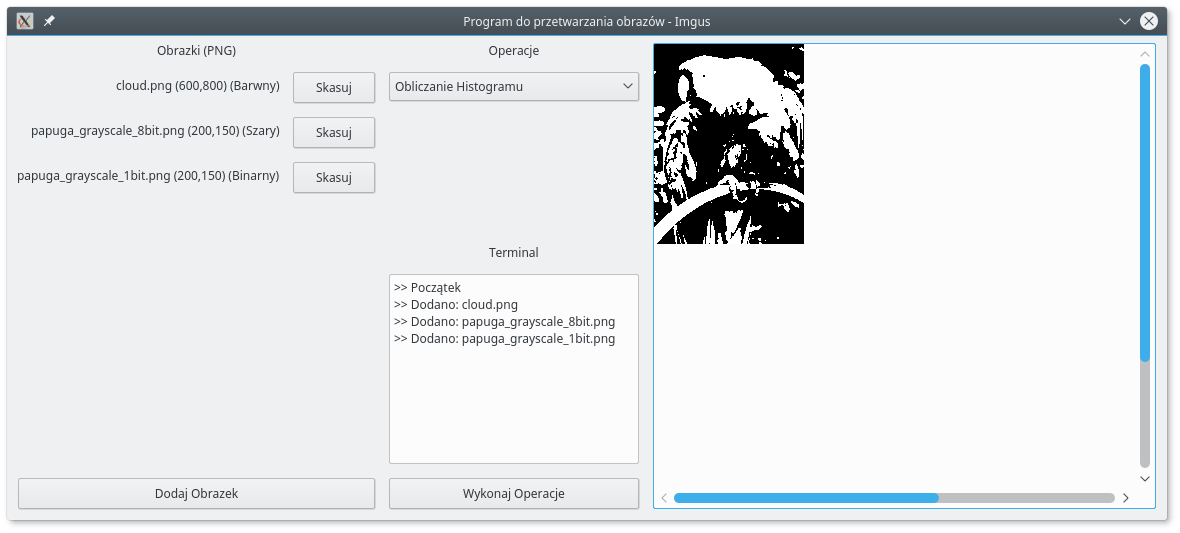
\includegraphics[scale=0.4]{img/example.png} 
\caption{Przykładowe wyświetlenie obrazów w programie.}
\label{fig:verticalcell}
\end{figure}

\FloatBarrier
\section{Najważniejsze Klas/Metod}
\subsection{Klasy Obiektów wykorzystywane w programu}
\begin{itemize}
\item {\bfseries Binary}{\itshape : extend(PointType*)} {\itshape (bool)} - Obiekt prezentuje piksel binarny który może mieć wartość równą 0 albo 1. Ma zmienną składową o nazwie 'pixel'.
\item {\bfseries GrayScale}{\itshape : extend(PointType*)} {\itshape (unsigned char)} -Obiekt prezentuje piksel o skali szarości z przedziałem 0-255. Ma zmienną składową o nazwie 'scale'.
\item {\bfseries RedGreenBlue}{\itshape : extend(PointType*)} {\itshape (unsigned char[3])} - Obiekt prezentuje piksel rgb mający 3 kanały z przedziałem 0-255, pierwszy kanał prezentuje czerwień, drugi zieleń, trzeci kolor niebieski. Ma zmienne składowe o nazwie 'red','green', 'blue'.
\item {\bfseries TemporaryImage} {\itshape (height, width, PointType*)} - Obiekt prezentuje tymczasowy obraz. Tak naprawdę jest to tylko wrapper vectora[height][width] o wartościach typów którego się podaje jako parametr.
\item {\bfseries Image} {\itshape (String fileName)} - Główny obiekt który zawiera obiekt składowy TemporaryImage przechowujący obraz oraz metody dzięki którym można operować nad tym obrazem. W Konstruktorze klasy jest przeprowadzana analiza nagłówka i dekodowanie obrazu do TemporaryImage i po zakończeniu operacji następuje enkodowanie.  
\end{itemize}
\subsection{Metody klas Binary/GrayScale/RedGreenBlue}
\begin{itemize}
\item {\bfseries set} {\itshape (PointType*)} - Funkcja która kopiuje wartości z piksela (parametr) do piksela bazowego. 
\item {\bfseries setBlank} {\itshape ()} - Funkcja która ustawia w przypadku Binary.pixel = false, w przypadku GrayScale.scale = 255, a w przypadku barwnych RedGreenBlue.red = 255, RedGreenBlue.green = 255, RedGreenBlue.blue = 255.
\end{itemize}
\subsection{Metody klasy TemporaryImage}
\begin{itemize}
\item {\bfseries operator()} {\itshape (int x, int y)} - przeciążenie operator () dla obiektu Temporary Image po wywołaniu operatora obiekt zwraca piksel typu PointType* z współrzędnych (x,y).
\end{itemize}
\subsection{Metody klasy Image}
\begin{itemize}
\item {\bfseries forEach} {\itshape (lambda)} - dzięki tej funkcji można dla każdego piksela wykonać jakieś działanie, operacje przeprowadzane na pikselu są zdefiniowane w funkcji lambda którą się przekazuje jako argument. Parametrem lambdy jest jawny PointType*. Lambdy pojawiły się w standardzie C++11.
\item {\bfseries cutFragment} {\itshape (width, height, x, y)} - dzięki tej funkcji można wyciąć fragment obrazu, funkcja zwraca obiekt TemporaryImage przedstawiający wycięty fragment.
\item {\bfseries copyFragment} {\itshape (TemporaryImage, x, y)} - funkcja kopiuje zawartość TemporaryImage w współrzędne (x,y) obrazu.
\item {\bfseries geometricAction} {\itshape (lambda)} - dzięki tej funkcji można przeprowadzić operacje przekształcające obraz, do funkcji przekazuje się lambdę która zawiera operacje przekształcające współrzędne. Parametrami lambdy są x i y. Po wykonaniu przekształcenia obraz jest zapisywany jako nowy TemporaryImage który później jest kopiowany do oryginalnego obrazka ( copyFragment() ).
\item {\bfseries morphologyOperation} {\itshape (lambda)} - dzięki tej funkcji można przeprowadzić operacje morfologiczne. Parametrem lambdy jest macierz 3x3 (bądź większa) prezentująca część obrazu. Po wykonaniu operacji w funkcji, lambda powinna zwrócić jawny PointType* który będzie nowym środkiem macierza którego się dostało jako parametr w lambdy.

\item {\bfseries minMax} {\itshape ()} - Funkcja zwracająca największą wartość i najmniejszą wartość w obrazie. Typ zwracany jest vector unsigned char
\item {\bfseries normalization} {\itshape ()} - Normalizuje obraz na podobnej zasadzie co operacja rozciąganie histogramu.
\item {\bfseries type} {\itshape ()} - Funkcja zwracająca informacje czy dany obraz jest typu Binary, GrayScale czy RGB.
\end{itemize}
\FloatBarrier
\section{Listing Operacje}
Każda funkcja operacji ma nazwę 'operate', to jest nic w tym dziwnego ponieważ te funkcje są w środku klasy które dziedziczą od klasy Operation która narzuca nam żeby funkcja operacji miała nazwę 'operate'. Za to nazwa klasy może się już różnić od innych: "Sum", "Blending", "Erosion" ...itd
\FloatBarrier
\subsection{Sumowanie}
Pierwsza funkcja operate przedstawia sumowanie dwóch obrazów. Za to druga przedstawia sumowanie przez stałą. Po każdym dodaniu piksela sprawdzany jest czy wartość nie przekroczyła przedziału 0-255. Operacja działa dla szarych i barwnych obrazów. Stała może być tylko Integer.
\begin{equation*}
f_(x,y)_{new} = f_(x,y)_{old}+g_(x,y)
\end{equation*}
\begin{equation*}
f_(x,y)_{new} = f_(x,y)_{old}+stala
\end{equation*}\\
\begin{Verbatim}[frame=single,label=Sumowanie (Source Code)]

    void operate (ImagePack pack, ParamsPack params)
    {
      Image *first = pack[0]; //pierwszy obraz
      Image *second = pack[1]; //drugi obraz

      first->forEach <GrayScale> (second,
        [](GrayScale *pt1, GrayScale *pt2){
        
          pt1->scale = pt1->scale + pt2->scale;
        }
      );

      first->forEach <RedGreenBlue> (second,
        [](RedGreenBlue *pt1, RedGreenBlue *pt2){
        
          pt1->red = pt1->red + pt2->red;
          pt1->green = pt1->green + pt2->green;
          pt1->blue = pt1->blue + pt2->blue;
        }
      );
    } 
    
    void operate (Image *img, ParamsPack params)
    {
      const int64_t stala = convertToNumber(params["Stała"]);

      img->forEach<GrayScale>([stala](GrayScale *pt){
      
          pt->scale = pt->scale + stala;
      });

      img->forEach<RedGreenBlue>([stala](RedGreenBlue *pt){
      
          pt->red = pt->red + stala;
          pt->green = pt->green + stala;
          pt->blue = pt->blue + stala;
      });
    }
       
\end{Verbatim}
\begin{figure}[!htb]
\centering
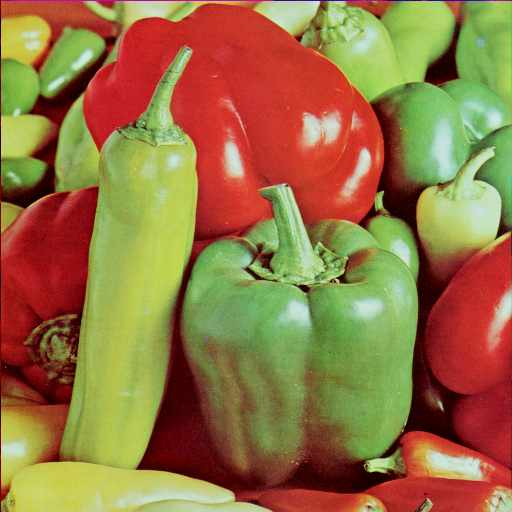
\includegraphics[scale=0.2]{img/peppers_24bit.png}
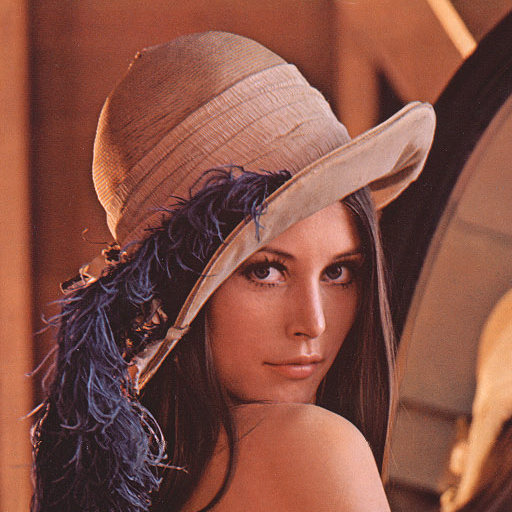
\includegraphics[scale=0.269]{img/lena_24bit.png} 
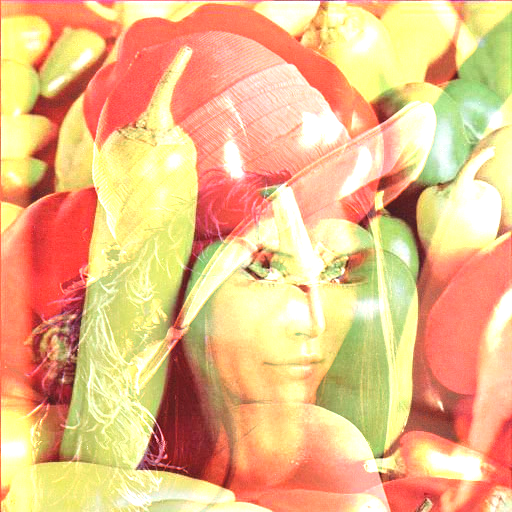
\includegraphics[scale=0.2]{img/_Sumowanie_Obrazka__lena_24bit_peppers_24bit.png}\\
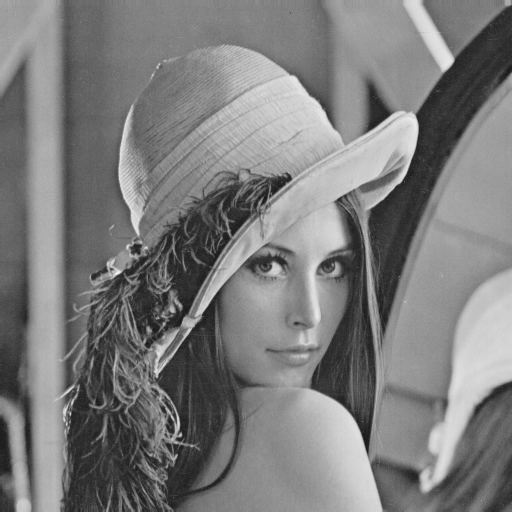
\includegraphics[scale=0.2]{img/lena_8bit.png} 
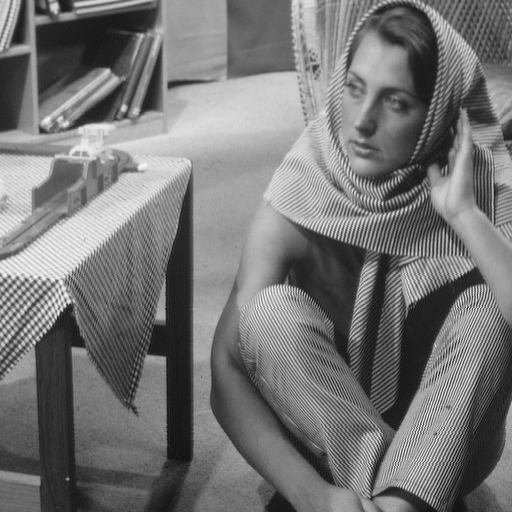
\includegraphics[scale=0.2]{img/barbara_8bit.png} 
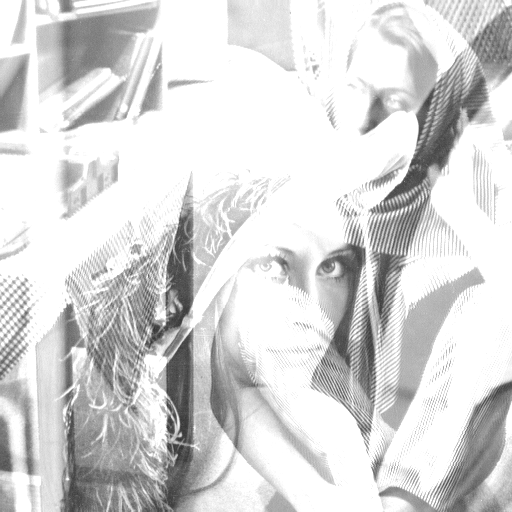
\includegraphics[scale=0.2]{img/_Sumowanie_Obrazka__barbara_8bit_lena_8bit.png}
\caption{Przykłady wykonania operacji sumowanie na obrazach - po lewej obraz przed operacją, po prawej obraz po operacji. }
\label{fig:verticalcell}
\end{figure}
\begin{figure}[!htb]
\centering
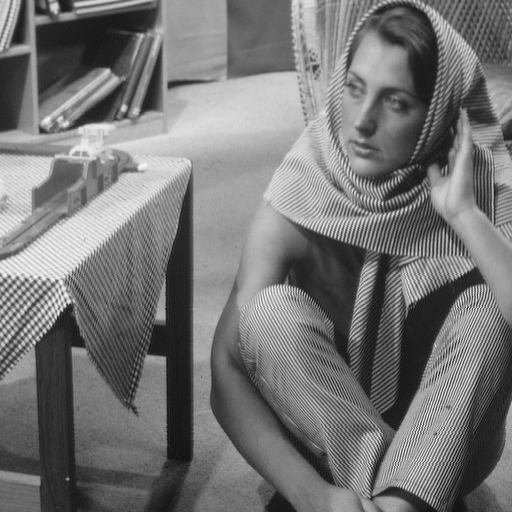
\includegraphics[scale=0.2]{img/barbara_8bit.png} 
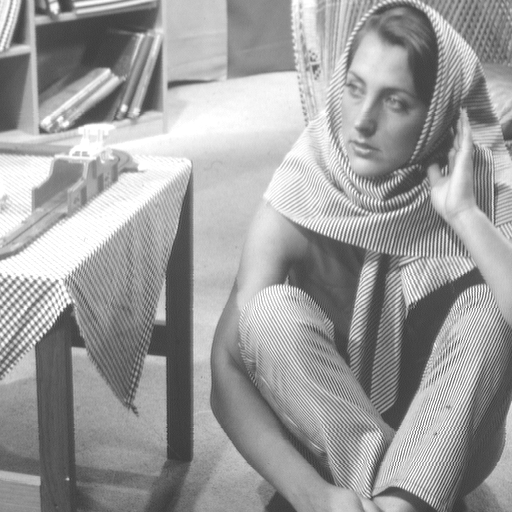
\includegraphics[scale=0.2]{img/_Sumowanie_Obrazka_barbara_8bit.png}
\caption{Przykłady wykonania operacji sumowania, stała to 40 - po lewej obraz przed operacją, po prawej obraz po operacji. }
\label{fig:verticalcell}
\end{figure}

\FloatBarrier
\subsection{Mnożenie}
Pierwsza funkcja operate przedstawia mnożenie dwóch obrazów. Za to druga przedstawia mnożenie przez mnożnik. Operacja ogranicza się tylko do obrazów szarych. Mnożnik może być tylko Integer.
\begin{equation*}
f_(x,y)_{new} = f_(x,y)_{old}*g_(x,y)
\end{equation*}
\begin{equation*}
f_(x,y)_{new} = f_(x,y)_{old}*mnoznik
\end{equation*}\\
\begin{Verbatim}[frame=single,label=Mnożenie (Source Code)]
    
    void operate (Image *img, ParamsPack params)
    {
      const uint64_t mnoznik = convertToNumber(params["Mnożnik"]);

      img->forEach<GrayScale>([mnoznik](GrayScale *pt){
      
          pt->scale = pt->scale * mnoznik;
      });
    }

    void operate (ImagePack pack, ParamsPack params)
    {
      Image *first = pack[0]; //pierwszy obraz
      Image *second = pack[1]; //drugi obraz

      first->forEach <GrayScale> (second,
        [](GrayScale *pt1, GrayScale *pt2){
        
          pt1->scale = pt1->scale * pt2->scale;
        }
      );
    }
    
\end{Verbatim}
\begin{figure}[!htb]
\centering
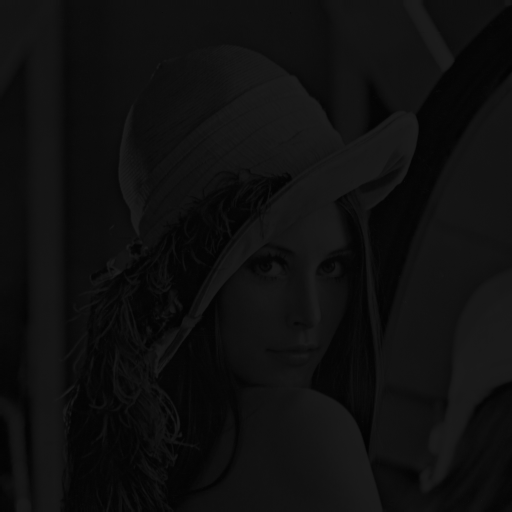
\includegraphics[scale=0.2]{img/dark_lena_8bit.png} 
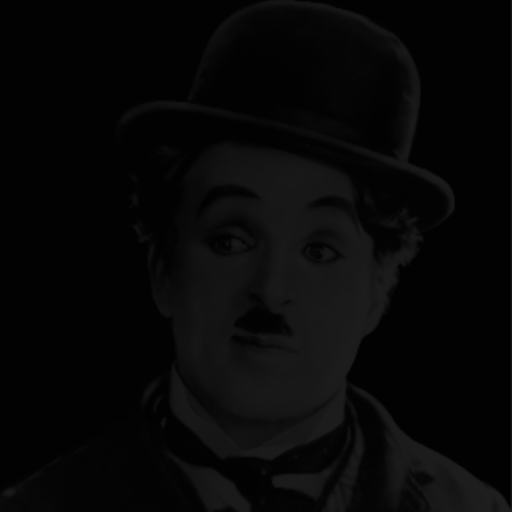
\includegraphics[scale=0.2]{img/dark_gray.png} 
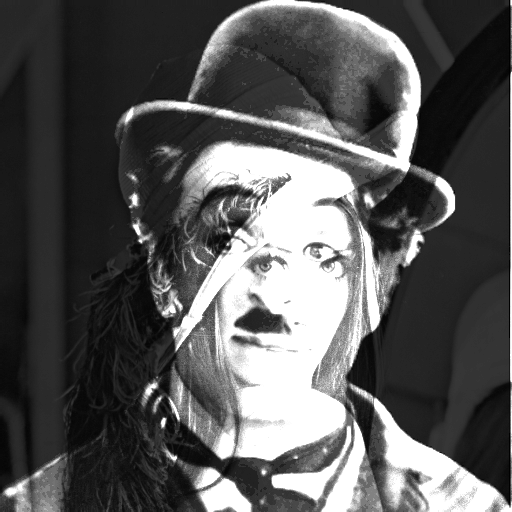
\includegraphics[scale=0.2]{img/_Mnozenie_Obrazka__lena_8bit_gray.png} 
\caption{Przykłady wykonania operacji mnożenia na obrazach - po lewej obraz przed operacją, po prawej obraz po operacji. }
\end{figure}
\begin{figure}[!htb]
\centering
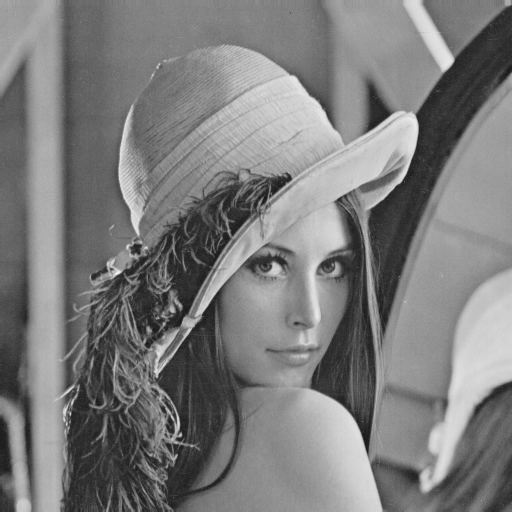
\includegraphics[scale=0.2]{img/lena_8bit.png} 
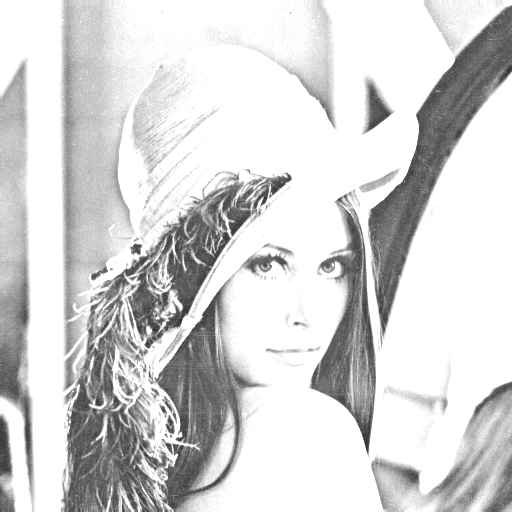
\includegraphics[scale=0.2]{img/_Mnozenie_Obrazka_lena_8bit.png}  
\caption{Przykłady wykonania operacji mnożenie, mnożnik to 2 - po lewej obraz przed operacją, po prawej obraz po operacji. }
\end{figure}

\FloatBarrier
\subsection{Mieszanie}
Funkcja operate przedstawia mieszanie dwóch obrazów. Operacje można przeprowadzić na obrazach szarych i barwnych. Wspolczynnik może być tylko Integer.
\begin{equation*}
f_(x,y)_{new} = wspolczynik*f_(x,y)_{old}+(1-wspolczynik)*g_(x,y)
\end{equation*}\\
\begin{Verbatim}[frame=single,label=Mieszanie (Source Code)]

    void operate (ImagePack pack, ParamsPack params)
    {
      Image *first = pack[0]; //pierwszy obraz
      Image *second = pack[1]; //drugi obraz

      const int64_t wsp = convertToNumber(params["Współczynnik"]);

      first->forEach <GrayScale> (second,
        [wsp](GrayScale *pt1, GrayScale *pt2){
        
        	pt1->scale = (wsp*pt1->scale) + ((1-wsp)*pt2->scale);
        }
      );

      first->forEach <RedGreenBlue> (second,
        [wsp](RedGreenBlue *pt1, RedGreenBlue *pt2){
        	
        	pt1->red = (wsp*pt1->red) + ((1-wsp)*pt2->red);
        	pt1->green = (wsp*pt1->green) + ((1-wsp)*pt2->green);
       	    pt1->blue = (wsp*pt1->blue) + ((1-wsp)*pt2->blue);
        }
      );
    }

\end{Verbatim}
\begin{figure}[!htb]
\centering
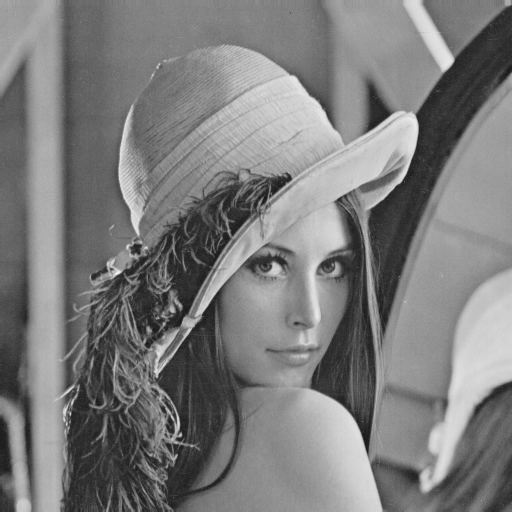
\includegraphics[scale=0.2]{img/lena_8bit.png}
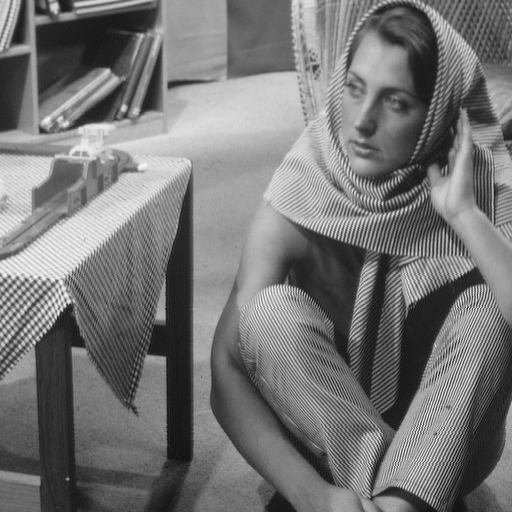
\includegraphics[scale=0.2]{img/barbara_8bit.png}   
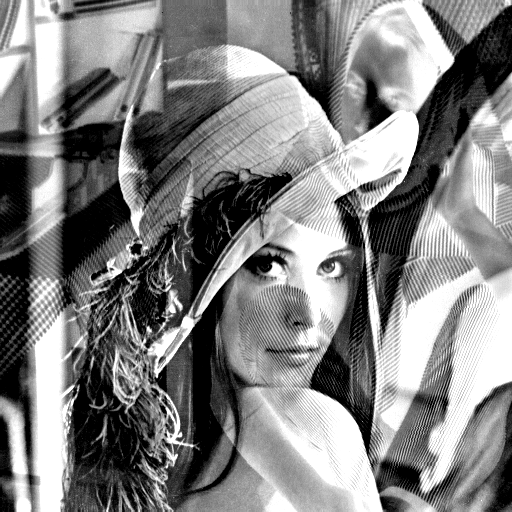
\includegraphics[scale=0.2]{img/_Mieszanie_Obrazow__lena_8bit_barbara_8bit.png}\\ 
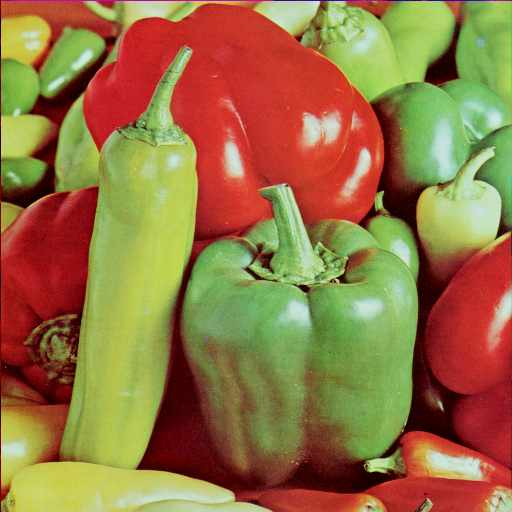
\includegraphics[scale=0.2]{img/peppers_24bit.png}
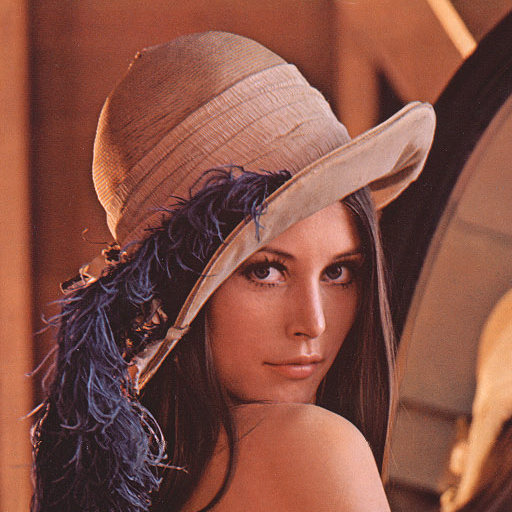
\includegraphics[scale=0.269]{img/lena_24bit.png}  
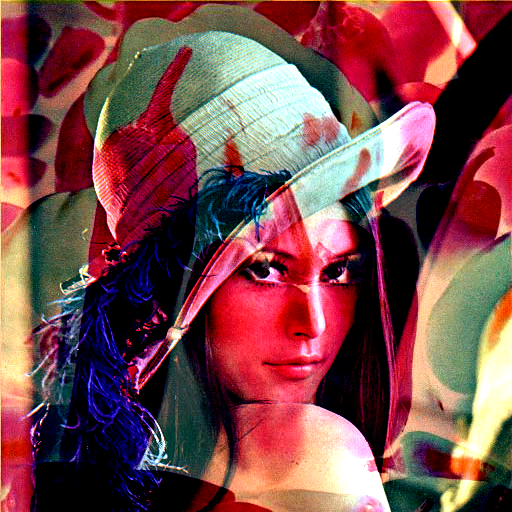
\includegraphics[scale=0.2]{img/_Mieszanie_Obrazow__lena_24bit_peppers_24bit.png}
\caption{Przykłady wykonania operacji Mieszanie z współczynnikiem 2 - po lewej obraz przed operacją, po prawej obraz po operacji. }
\end{figure}

\FloatBarrier
\subsection{Potęgowanie}
Funkcja operate przedstawia potęgowanie obrazu. Operacje można przeprowadzić na obrazach szarych i barwnych. Potęga może być tylko Integer. Po każdej operacji na pikselu, obraz będzie się normalizował.
\begin{equation*}
f_(x,y)_{new} = 255*(\frac{f_(x,y)_{old}}{MaxValue})^{potega}
\end{equation*}\\
\begin{Verbatim}[frame=single,label=Potęgowanie (Source Code)]

    void operate (Image *img, ParamsPack params)
    {
      const uint64_t potega = convertToNumber(params["Potęga"]);

      vector <unsigned char> minMax = img->minMax();

      img->forEach<GrayScale>([&](GrayScale *pt){
      
          pt->scale = 255.0 * pow((pt->scale) / (minMax[1]), potega);
      });

      img->forEach<RedGreenBlue>([&](RedGreenBlue *pt){
      
          pt->red = 255.0 * pow((pt->red) / (minMax[3]), potega);
          pt->green = 255.0 * pow((pt->green) / (minMax[4]), potega);
          pt->blue = 255.0 * pow((pt->blue) / (minMax[5]), potega);
      });
    }
    
\end{Verbatim}
\begin{figure}[!htb]
\centering
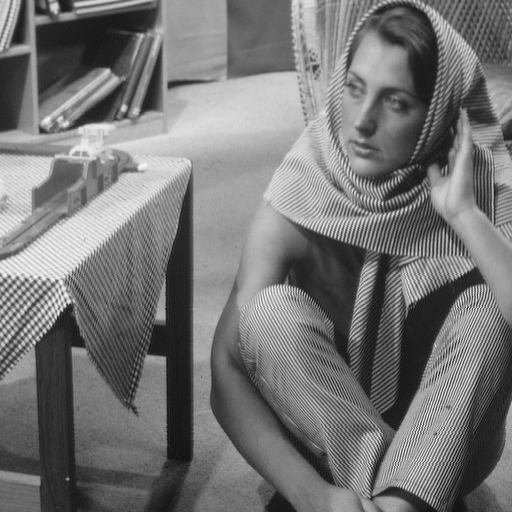
\includegraphics[scale=0.2]{img/barbara_8bit.png} 
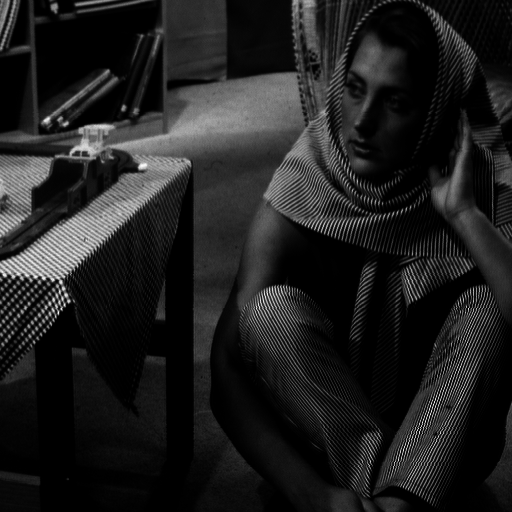
\includegraphics[scale=0.2]{img/Potegowanie_Obrazu_barbara_8bit.png}\\
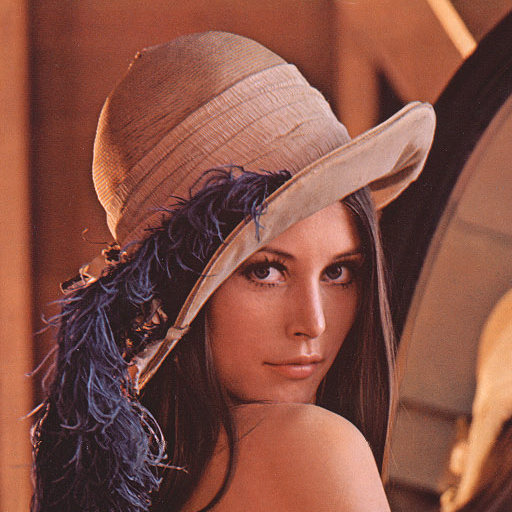
\includegraphics[scale=0.269]{img/lena_24bit.png}  
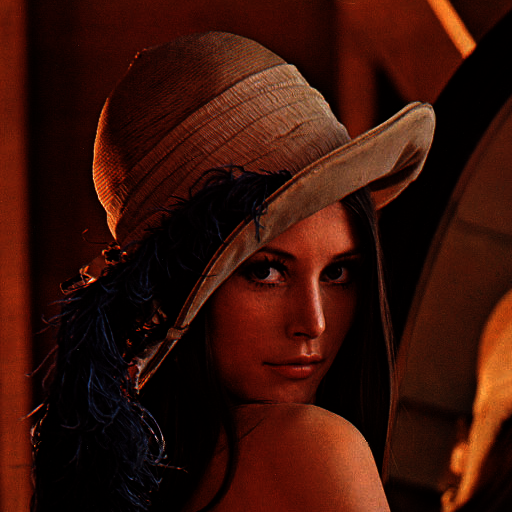
\includegraphics[scale=0.2]{img/Potegowanie_Obrazu_lena_24bit.png} 
\caption{Przykłady wykonania operacji potęgowanie z potęgą 4 - po lewej obraz przed operacją, po prawej obraz po operacji. }
\end{figure}

\FloatBarrier
\subsection{Dzielenie}
Pierwsza funkcja operate przedstawia dzielenie dwóch obrazów. Za to druga przedstawia dzielenie przez dzielnik. Operacja ogranicza się tylko do obrazów szarych. Dzielnik może być tylko Integer.
Po wykonaniu dzielenia, jest wykonywana normalizacja.
\begin{equation*}
f_(x,y)_{new} = \frac{f_(x,y)_{old}}{g_(x,y)}
\end{equation*}
\begin{equation*}
f_(x,y)_{new} = \frac{f_(x,y)_{old}}{dzielnik}
\end{equation*}\\
\begin{Verbatim}[frame=single,label=Dzielenie (Source Code)]

      void operate (Image *img, ParamsPack params)
      {
        const uint64_t dzielnik = convertToNumber(params["Dzielnik"]);

        img->forEach<GrayScale>([dzielnik](GrayScale *pt){
        
            pt->scale = pt->scale / dzielnik;
        });
      }

      void operate (ImagePack pack, ParamsPack params)
      {
        Image *first = pack[0];
        Image *second = pack[1];

        first->forEach <GrayScale> (second,
          [&](GrayScale *pt1, GrayScale *pt2){
          
            pt1->scale = (pt1->scale) / ((pt2->scale != 0)?(pt2->scale):(1.0));
          }
        );

        first->normalization();
      }

\end{Verbatim}
\begin{figure}[!htb]
\centering
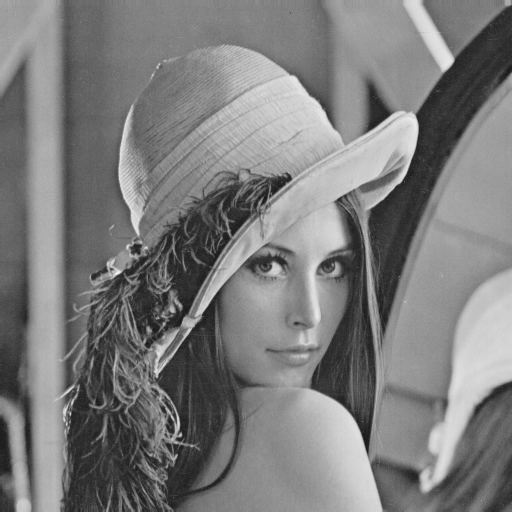
\includegraphics[scale=0.2]{img/lena_8bit.png}
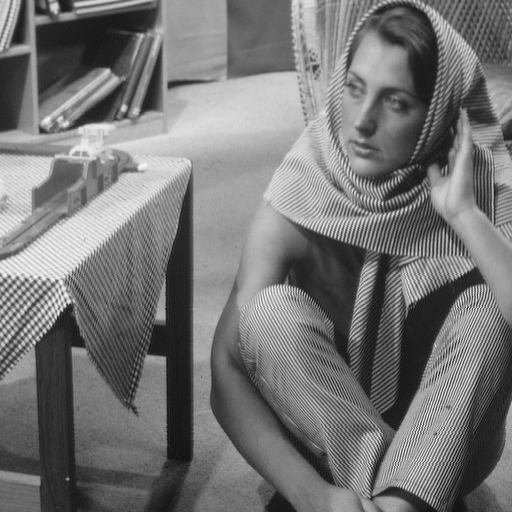
\includegraphics[scale=0.2]{img/barbara_8bit.png} 
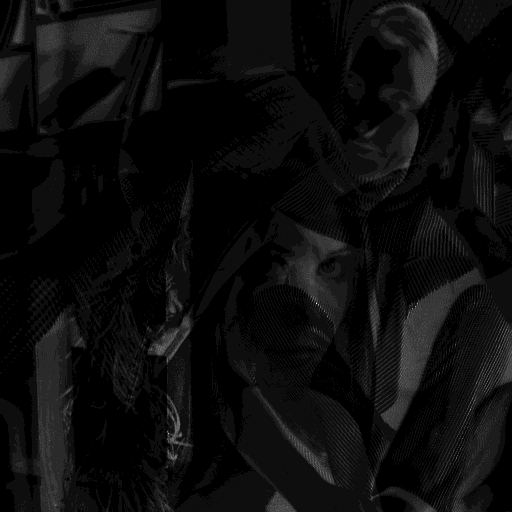
\includegraphics[scale=0.2]{img/_Dzielenie_Obrazka__lena_8bit_barbara_8bit.png} \\
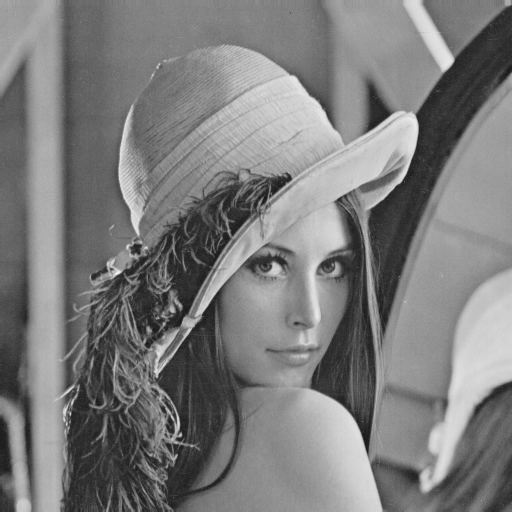
\includegraphics[scale=0.2]{img/lena_8bit.png}
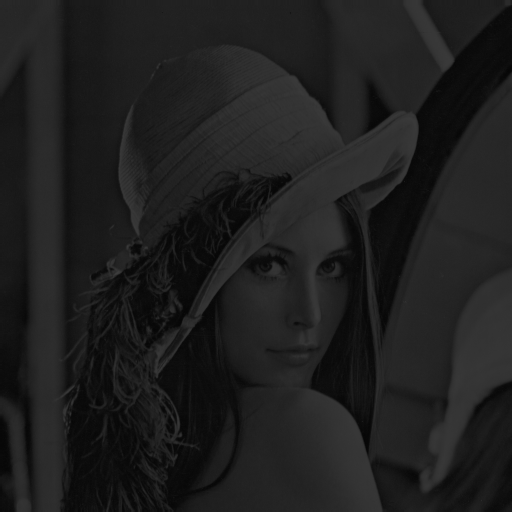
\includegraphics[scale=0.2]{img/_Dzielenie_Obrazka_lena_8bit.png} 
\caption{Przykłady wykonania operacji dzielenia z dwoma obrazami i z dzielnikiem równym 4 - po lewej obraz przed operacją, po prawej obraz po operacji. }
\end{figure}

\FloatBarrier
\subsection{Pierwiastkowanie}
Funkcja operate przedstawia pierwiastkowanie obrazu. Operacje można przeprowadzić na obrazach szarych i barwnych. Po każdej operacji na pikselu, obraz będzie się normalizował.
\begin{equation*}
f_(x,y)_{new} = 255*\sqrt{\frac{f_(x,y)_{old}}{MaxValue}}
\end{equation*}\\
\begin{Verbatim}[frame=single,label=Pierwiastkowanie (Source Code)]

    void operate (Image *img, ParamsPack params)
    {
      vector <unsigned char> minMax = img->minMax();

      img->forEach<GrayScale>([&](GrayScale *pt){
      
          pt->scale = 255.0 * sqrt(double(pt->scale)/double(minMax[1]));
      });

      img->forEach<RedGreenBlue>([&](RedGreenBlue *pt){
      
          pt->red = 255.0 * sqrt(double(pt->red) / double(minMax[3]));
          pt->green = 255.0 * sqrt(double(pt->green) / double(minMax[4]));
          pt->blue = 255.0 * sqrt(double(pt->blue) / double(minMax[5]));
      });
    }
    
\end{Verbatim}
\begin{figure}[!htb]
\centering
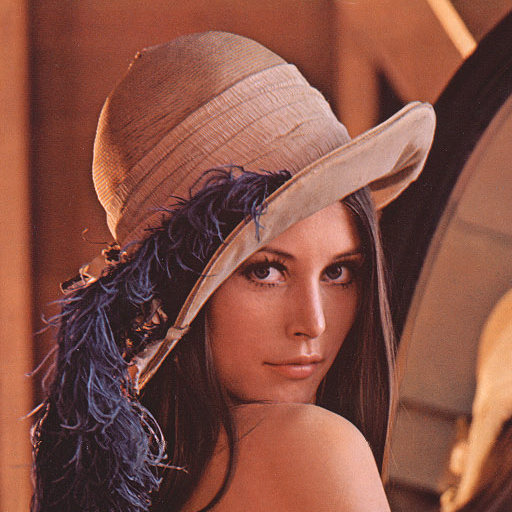
\includegraphics[scale=0.269]{img/lena_24bit.png} 
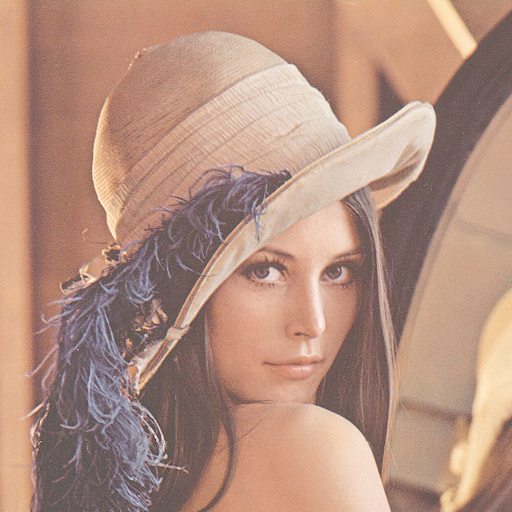
\includegraphics[scale=0.2]{img/_Pierwiastkowanie_Obrazu_lena_24bit.png}\\
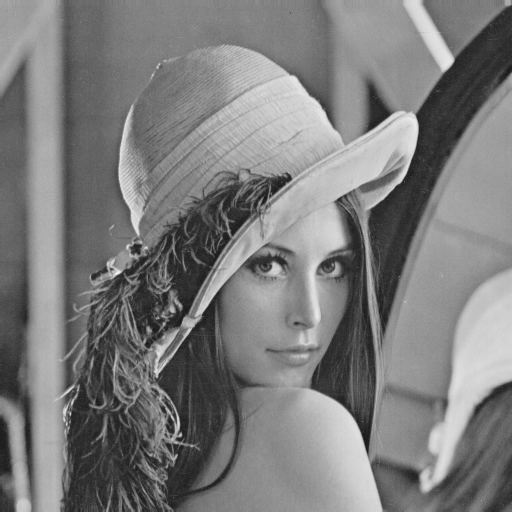
\includegraphics[scale=0.2]{img/lena_8bit.png}
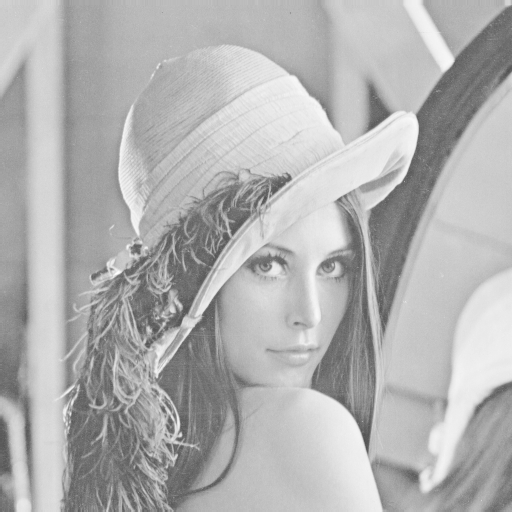
\includegraphics[scale=0.2]{img/_Pierwiastkowanie_Obrazu_lena_8bit.png} 
\caption{Przykłady wykonania operacji pierwiastkowanie - po lewej obraz przed operacją, po prawej obraz po operacji. }
\end{figure}

\FloatBarrier
\subsection{Logarytmowanie}
Funkcja operate przedstawia Logarytmowanie obrazu. Operacje można przeprowadzić na obrazach szarych i barwnych. Po każdej operacji na pikselu, obraz będzie się normalizował.
W logarytmie dodaje się 1, bo nie może być w log równe 0.
\begin{equation*}
f_(x,y)_{new} = 255*\frac{\log_{10}{(1+f_(x,y)_{old})}}{\log_{10}{(1+MaxValue)}}
\end{equation*}\\
\begin{Verbatim}[frame=single,label=Logarytmowanie (Source Code)]

 void operate (Image *img, ParamsPack params)
 {
  vector <unsigned char> minMax = img->MinMax();
	
  img->forEach<GrayScale>([&](GrayScale *pt){
  
     pt->scale = 255.0 * log10(1.0 + (pt->scale))/log10(1.0+(minMax[1]));
  });
	
  img->forEach<RedGreenBlue>([&](RedGreenBlue *pt){
  
     pt->red = 255.0 * log10(1.0 + (pt->red))/log10(1.0+(minMax[3]));
     pt->green = 255.0 * log10(1.0 + (pt->green))/log10(1.0+(minMax[4]));
     pt->blue = 255.0 * log10(1.0 + (pt->blue))/log10(1.0+(minMax[5]));
  });
 }
    
\end{Verbatim}
\begin{figure}[!htb]
\centering
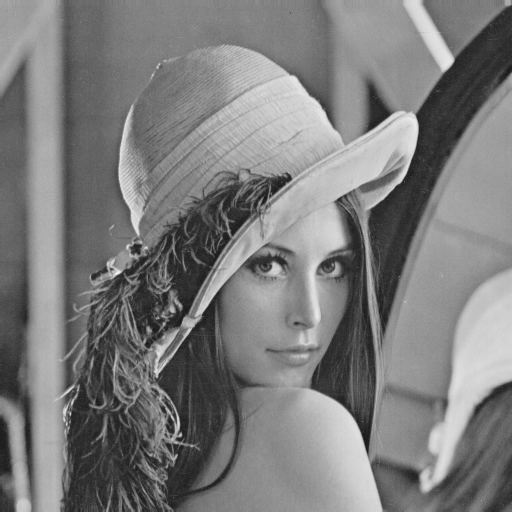
\includegraphics[scale=0.2]{img/lena_8bit.png}
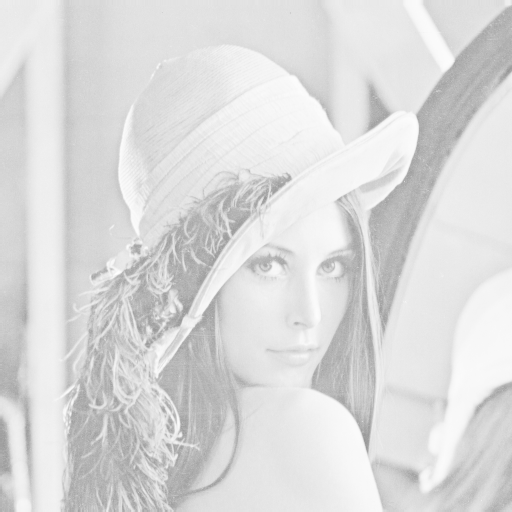
\includegraphics[scale=0.2]{img/_Logarytmowanie_Obrazu_lena_8bit.png}\\
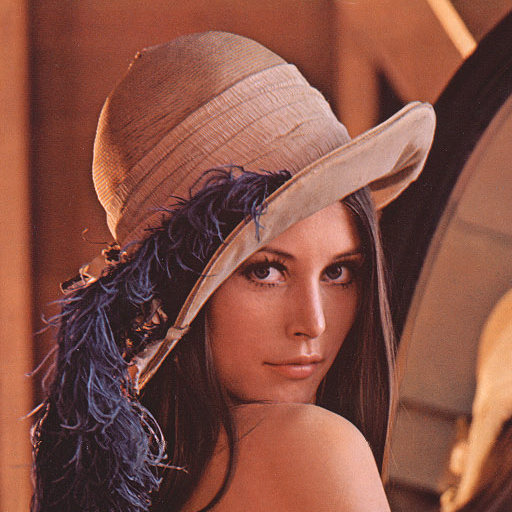
\includegraphics[scale=0.269]{img/lena_24bit.png} 
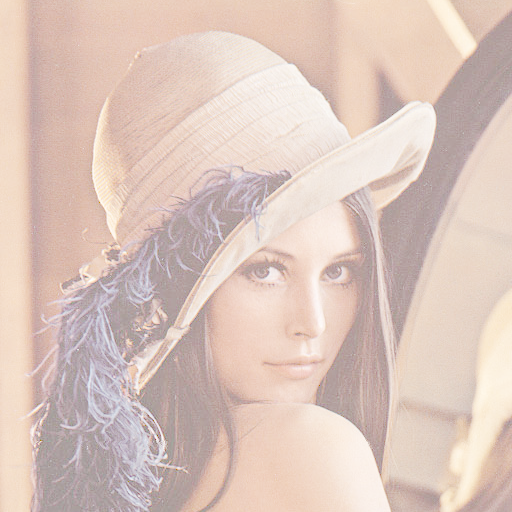
\includegraphics[scale=0.2]{img/_Logarytmowanie_Obrazu_lena_24bit.png} 
\caption{Przykłady wykonania operacji logarytmowania - po lewej obraz przed operacją, po prawej obraz po operacji. }
\end{figure}

\FloatBarrier
\subsection{Przemieszczanie Obrazu}
Funkcja operate przedstawia przemieszczenie się obrazka. Wystarczy podać wektor [x,y] który przeniesie każdy piksel pod nowe współrzędne.
\begin{equation*}
f_(x,y) = g_(x+x_{move},y+y_{move})
\end{equation*}\\
\begin{Verbatim}[frame=single,label=Przemieszczanie Obrazu (Source Code)]

    void operate(Image *img, ParamsPack params)
    {
      const uint64_t moveX = convertToNumber(params["X"]);
      const uint64_t moveY = convertToNumber(params["Y"]);

      img->geometricAction(
        [moveX,moveY] (uint64_t x, uint64_t y) -> Point_t
        {
          return Point_t { x + moveX, y + moveY };
        }
      );
    }
    
\end{Verbatim}
\begin{figure}[!htb]
\centering
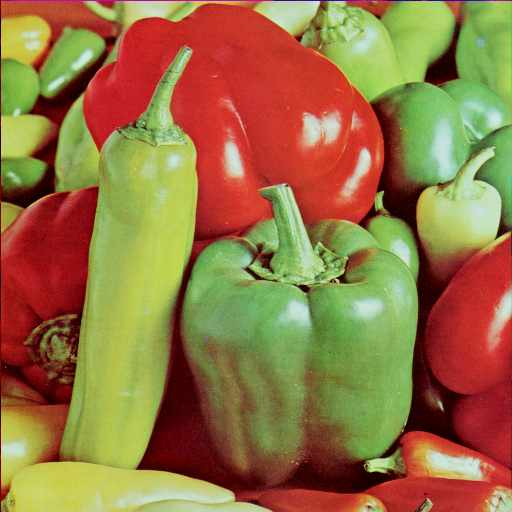
\includegraphics[scale=0.2]{img/peppers_24bit.png}
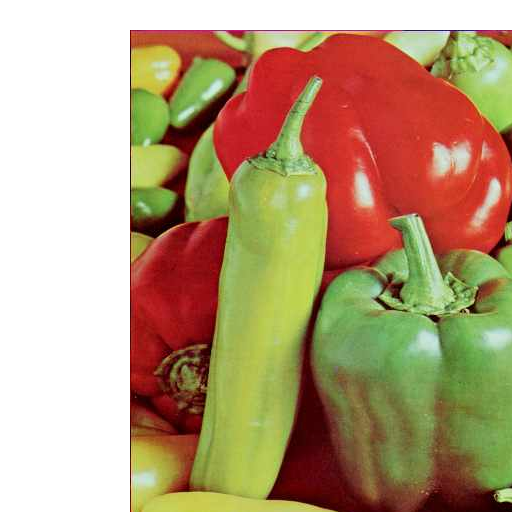
\includegraphics[scale=0.2]{img/Przemieszczenie_Obrazu_peppers_24bit.png} 
\caption{Przykłady wykonania operacji przemieszczenie obrazu x = 30, y = 10 - po lewej obraz przed operacją, po prawej obraz po operacji. }
\end{figure}

\FloatBarrier
\subsection{Wycinanie Fragmentu Obrazu}
Funkcja operate przedstawia wycinanie fragmentu obrazu. Wystarczy podać współrzędne wycięcia (x,y) i podać również jak duży ma być wycięty fragment.
\begin{Verbatim}[frame=single,label=Wycinanie Fragmentu Obrazu (Source Code)]

    void operate (Image *img, ParamsPack params)
    {
      const uint64_t startX = convertToNumber(params["X"]);
      const uint64_t startY = convertToNumber(params["Y"]);
      const uint64_t heigth = convertToNumber(params["Heigth"]);
      const uint64_t width = convertToNumber(params["Width"]);

      img->cutFragment(width, heigth, startX, startY);
    }

\end{Verbatim}
\begin{figure}[!htb]
\centering
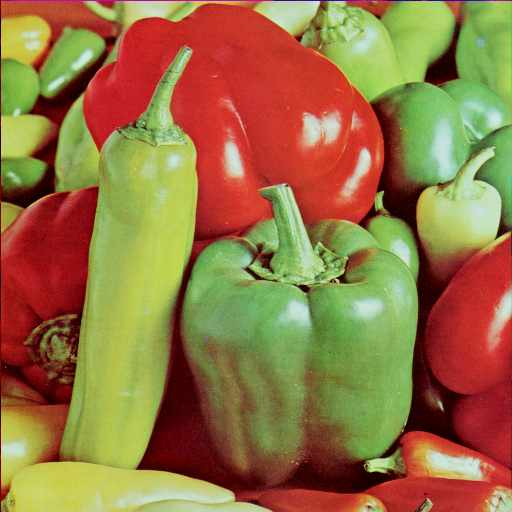
\includegraphics[scale=0.2]{img/peppers_24bit.png}
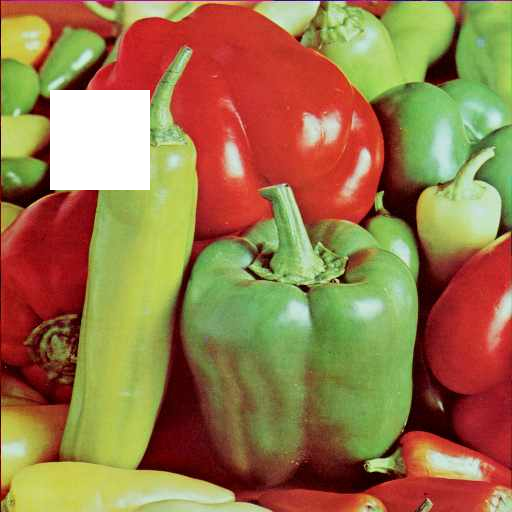
\includegraphics[scale=0.2]{img/Wyciety_Fragment_Obraz_peppers_24bit.png} 
\caption{Przykłady wykonania operacji wycięcie fragmentu obrazu współrzędne (10,30) h = 30 w = 30 - po lewej obraz przed operacją, po prawej obraz po operacji. }
\end{figure}

\FloatBarrier
\subsection{Kopiowanie Fragmentu Obrazu}
Funkcja operate przedstawia wycinanie fragmentu obrazu. Wystarczy podać współrzędne wycięcia (x,y), współrzędne kopiowania (x2, y2) i jak wielki ma być fragment obrazu.
\begin{Verbatim}[frame=single,label=Kopiowanie Fragmentu Obrazu (Source Code)]

    void operate(Image *img, ParamsPack params)
    {
      const uint64_t startX = convertToNumber(params["X"]);
      const uint64_t startY = convertToNumber(params["Y"]);
      const uint64_t heigth = convertToNumber(params["Heigth"]);
      const uint64_t width = convertToNumber(params["Width"]);
      const uint64_t pasteX = convertToNumber(params["X2"]);
      const uint64_t pasteY = convertToNumber(params["Y2"]);
	
      TemporaryImage tmpImg = img->cutFragment(width, heigth, startX, startY);
      img->copyFragment(tmpImg, pasteX, pasteY);
    }

\end{Verbatim}
\begin{figure}[!htb]
\centering
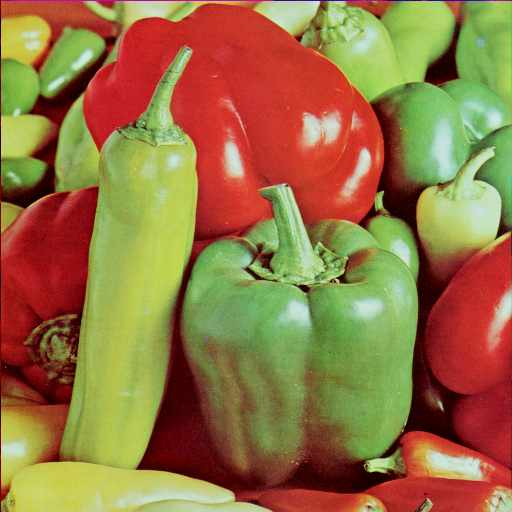
\includegraphics[scale=0.2]{img/peppers_24bit.png}
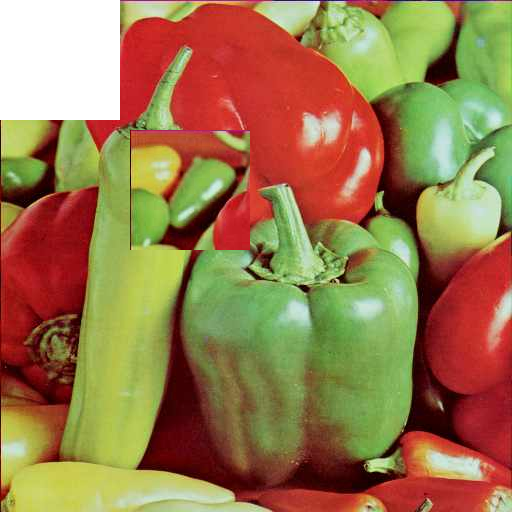
\includegraphics[scale=0.2]{img/Kopiuj_Wklej_Obraz_peppers_24bit.png} 
\caption{Przykłady wykonania operacji kopiowanie fragmentu obrazu z (0,0) do (60,60) h = 50 w = 50 - po lewej obraz przed operacją, po prawej obraz po operacji. }
\end{figure}

\FloatBarrier
\subsection{Obliczanie Histogramu}
Operacja wyświetla histogram obrazka. To działa dla obrazów szarych i barwnych. W przypadku obrazów barwnych pokazują się 3 histogramy dla czerwonego, zielonego, niebieskiego.
\begin{figure}[!htb]
\centering
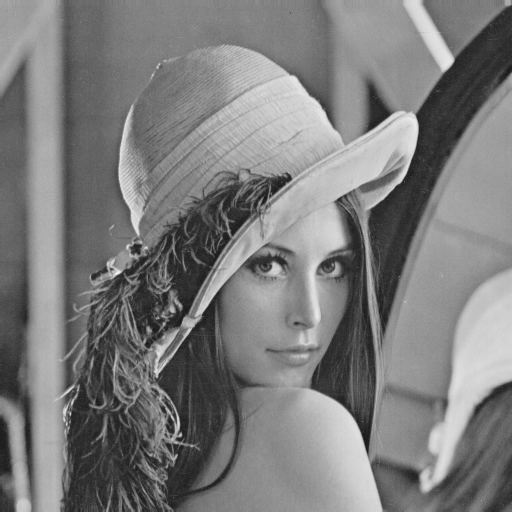
\includegraphics[scale=0.2]{img/lena_8bit.png}
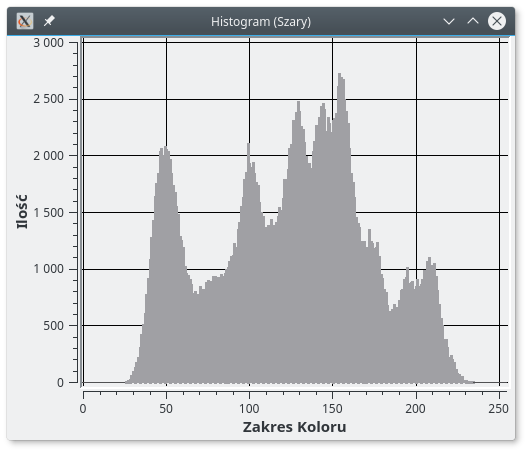
\includegraphics[scale=0.3]{img/histogram.png} 
\caption{Przykłady wykonania operacji wyświetlenie histogramu - po lewej obraz a po prawej histogram obrazu. }
\end{figure}

\FloatBarrier
\subsection{Rozciąganie Histogramu}
Operacja rozciąga histogram.  To działa dla obrazów szarych i barwnych. Dla każdego piksela wykonuje się formułę:
\begin{equation*}
f_(x,y)_{new} = 255* \frac{f_(x,y)_{old}-MinValue}{MaxValue-MinValue}
\end{equation*}\\
\begin{figure}[!htb]
\centering
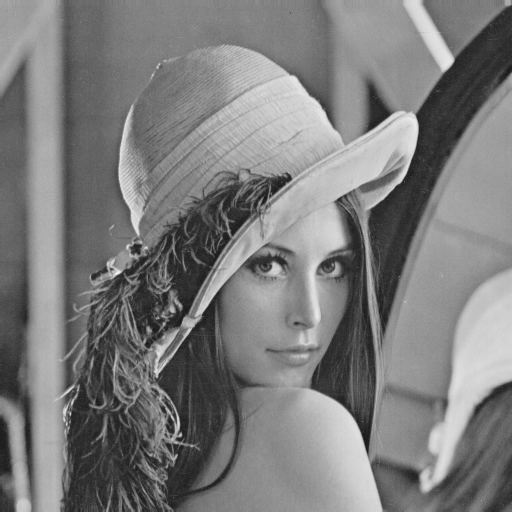
\includegraphics[scale=0.2]{img/lena_8bit.png}
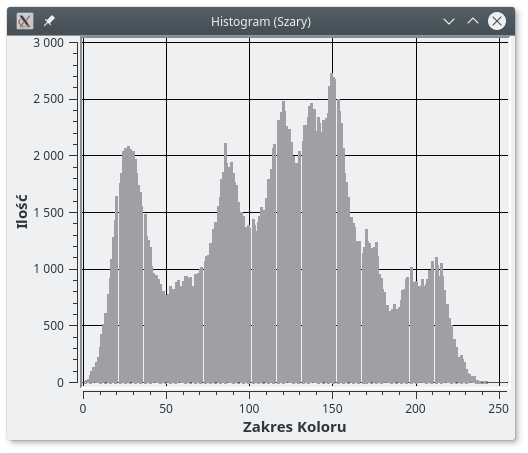
\includegraphics[scale=0.3]{img/histogram-rozciaganie.png} 
\caption{Przykłady wykonania operacji rozciąganie histogramu - po lewej obraz a po prawej histogram obrazu. }
\end{figure}

\FloatBarrier
\subsection{Progowanie Lokalne}
Funkcja operate przezentuję progowanie lokalne. Dla każdego piksela jest pobierany macierz 7x7 i w nim jest obliczany thresholding lokalny dzięki formule:
\begin{equation*}
T_(x,y) =  \frac{MaxValue + MinValue}{2}
\end{equation*}
Później jest porównywany z środkowym pikselem macierza:
\begin{equation*}
F_(x,y)_{new} =  \begin{cases}1 \mbox{ if } f(x,y)_{old} > T_(x,y) \\ 0 \mbox{ if } f(x,y)_{old} \leq T_(x,y)\end{cases}
\end{equation*}
Po operacji obrazy szare są zmieniane w obrazy binarne. W przypadku obrazów barwnych, są pierw zmieniane na obrazy szare a później na obrazy binarne. Do tego jest wykorzystywana funkcja RGBtoGrayScale. \\
\begin{Verbatim}[frame=single,label=Progowanie Lokalne (Source Code)]

    unsigned char RGBtoGrayScale (float R, float G, float B)
    {
      return (0.21*R + 0.72*G + 0.07*B);
    }

    void operate(Image *img, ParamsPack params)
    {
	vector <unsigned char> minMax = img->minMax();    
    
        img->morphologyOperation<GrayScale, 7>(
          [](GrayScale* pixelStructure[49]) -> PointType* {
	
		// pixelStructure[9] to macierz 7x7 obrazu dla piksela (x, y)		

            if (pixelStructure[24]->scale > ((minMax[1]+minMax[0])/2))
              return (new GrayScale(255));
            else
              return (new GrayScale(0));
          }
        );

        img->morphologyOperation<RedGreenBlue, 7>(
          [this](RedGreenBlue* pixelStructure[49]) -> PointType* {
			
		// pixelStructure[9] to macierz 7x7 obrazu dla piksela (x, y)			
			
            unsigned char min = 255;
            unsigned char max = 0;
			
			// szukanie min i max
            for(int i = 0; i < 49; ++i)
            {
              if (pixelStructure[i])
              {
                unsigned char intensity = RGBtoGrayScale(
                	pixelStructure[i]->red, 
                	pixelStructure[i]->green, 
                	pixelStructure[i]->blue
                );
                if (intensity < min) min = intensity;
                if (intensity > max) max = intensity;
              }
            }     
            
            unsigned char middle = RGBtoGrayScale(
           		pixelStructure[24]->red, 
            	pixelStructure[24]->green, 
            	pixelStructure[24]->blue
            );
            if (middle > ((max+min)/2))
              return (new RedGreenBlue(255,255,255));
            else
              return (new RedGreenBlue(0,0,0));
          }
        );
    }

\end{Verbatim}
\begin{figure}[!htb]
\centering
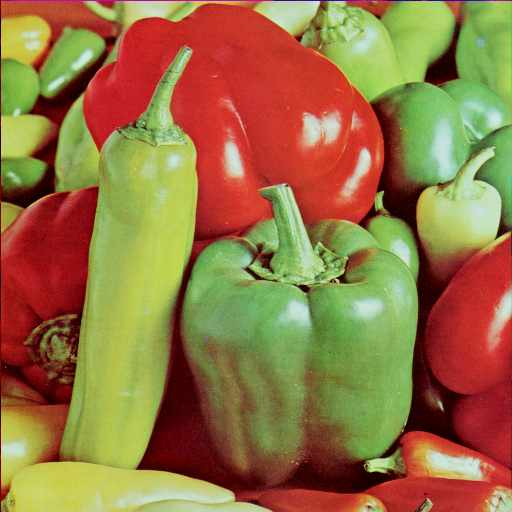
\includegraphics[scale=0.2]{img/peppers_24bit.png}
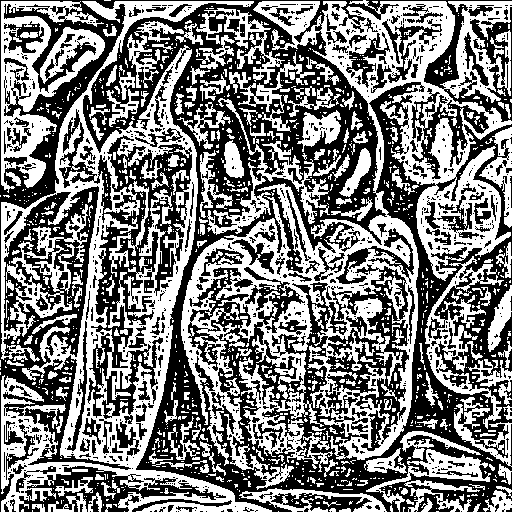
\includegraphics[scale=0.2]{img/Progowanie_Lokalne_peppers_24bit.png}\\
\includegraphics[scale=0.2]{img/lena_8bit.png} 
\includegraphics[scale=0.2]{img/Progowanie_Lokalne_lena_8bit.png} 
\caption{Przykłady wykonania operacji progowanie lokalne - po lewej obraz przed operacją, po prawej obraz po operacji. }
\end{figure}

\FloatBarrier
\subsection{Progowanie Globalne}
Progowanie globalne wykonuje się analogicznie jak progowanie lokalne tylko że thresholding jest ten sam dla każdego piksela. Jest tylko raz obliczany.
\begin{equation*}
T =  \frac{MaxValue + MinValue}{2}
\end{equation*}
\begin{equation*}
F_(x,y)_{new} =  \begin{cases}1 \mbox{ if } f(x,y)_{old} > T \\ 0 \mbox{ if } f(x,y)_{old} \leq T\end{cases}
\end{equation*}\\
\begin{Verbatim}[frame=single,label=Progowanie Globalne (Source Code)]
    
    unsigned char RGBtoGrayScale (float R, float G, float B)
    {
      return (0.21*R + 0.72*G + 0.07*B);
    }

    void operate(Image *img, ParamsPack params)
    {
    vector <unsigned char> minMax = img->minMax();
    	
      if (img->type() == POINT_TYPES::GRAY_SCALE)
      {
        unsigned char thresholding = (minMax[1]+minMax[0])/2;
        
        img->forEach <GrayScale> ([thresholding]( GrayScale *pt ){
        
            if (pt->scale > thresholding)
              pt->scale = 255;
            else
              pt->scale = 0;
        });
      }

      if (img->type() == POINT_TYPES::RGB)
      {
        unsigned char min = 255;
        unsigned char max = 0;
        
        img->forEach <RedGreenBlue> ([this,&min,&max]( RedGreenBlue *pt ){
        
            unsigned char intensity = RGBtoGrayScale(
            	pt->red, 
            	pt->green, 
            	pt->blue
            );
            if (min > intensity) min = intensity;
            if (max < intensity) max = intensity;
        });
        
        unsigned char thresholding = (max+min)/2;
        
        img->forEach <RedGreenBlue> ([this,thresholding]( RedGreenBlue *pt ){
            unsigned char intensity = RGBtoGrayScale(
            	pt->red, 
            	pt->green, 
            	pt->blue
            );
            if (intensity > thresholding)
            {
              pt->red = 255;
              pt->green = 255;
              pt->blue = 255;
            }
            else
            {
              pt->red = 0;
              pt->green = 0;
              pt->blue = 0;
            }
        });

      }
    }
    
\end{Verbatim}
\begin{figure}[!htb]
\centering
\includegraphics[scale=0.2]{img/peppers_24bit.png}
\includegraphics[scale=0.2]{img/Progowanie_Globalne_peppers_24bit.png}\\ 
\includegraphics[scale=0.2]{img/lena_8bit.png} 
\includegraphics[scale=0.2]{img/Progowanie_Globalne_lena_8bit.png} 
\caption{Przykłady wykonania operacji progowanie globalne - po lewej obraz przed operacją, po prawej obraz po operacji. }
\end{figure}

\FloatBarrier
\subsection{Progowanie Wieloprogowe}
Operacja progowanie wieloprogowe jest podobna do progowania lokalne i globalne tylko że operacja ta ma dwa threshold, które wyznaczają 3 przedziały i dla każdego przedziału jest wyróżniony piksel. Threshold'y podajemy przez parametry nie są wyliczane. Ja przyjąłem że kiedy wartość piksela jest miejsza od T1 to piksel jest czerwony, kiedy mieści się w przedziale jest zielony, a kiedy jest więszy od T2 to jest piksel niebieski.
\begin{equation*}
F_(x,y)_{new} =  \begin{cases}a \mbox{ if } f(x,y)_{old} > T_{1} \\ b \mbox{ if } T_{1} < f(x,y)_{old} \leq T_{2} \\ c \mbox{ if } f(x,y)_{old} \leq T_{2}\end{cases}
\end{equation*}\\
\begin{Verbatim}[frame=single,label=Progowanie Wieloprogowe (Source Code)]

    unsigned char RGBtoGrayScale (float R, float G, float B)
    {
      return (0.21*R + 0.72*G + 0.07*B);
    }

    void operate(Image *img, ParamsPack params)
    {
        const uint64_t T1 = convertToNumber(params["T1"]);
        const uint64_t T2 = convertToNumber(params["T2"]);

        img->forEach<RedGreenBlue>([this,T1,T2](RedGreenBlue *pt){
        
            unsigned char intensity = RGBtoGrayScale(
            	pt->red, 
            	pt->green, 
            	pt->blue
            );
            
            if (intensity < T1)
            {
              pt->red = 255;
              pt->green = 0;
              pt->blue = 0;
            }
            else if (T1 < intensity < T2)
            {
              pt->red = 0;
              pt->green = 255;
              pt->blue = 0;
            }
            else if (intensity > T2)
            {
              pt->red = 0;
              pt->green = 0;
              pt->blue = 255;
            }
        });
    }
    
\end{Verbatim}
\begin{figure}[!htb]
\centering
\includegraphics[scale=0.269]{img/lena_24bit.png} 
\includegraphics[scale=0.2]{img/Progowanie_Wieloprogowe_lena_24bit.png} 
\caption{Przykłady wykonania operacji progowanie wieloprogowe T1=90, T2=140 - po lewej obraz przed operacją, po prawej obraz po operacji. }
\end{figure}

\FloatBarrier
\subsection{Okrawanie (Erozja)}
Funkcja operate prezentuje operacje erozje. Dla zdjęć binarnych, dla każdego piksela sprawdzani są sąsiedzi (góra, dół, lewo, prawo) i jeśli jeden z tych sąsiadów ma wartość 0 to piksel na środku będzie miał też 0 jeśli nie to 1. W przypadku zdjęć szarych, w macierz 3x3 jest wyszukiwana najmniejsza wartość i ta wartość będzie wartością środkową piksela. Ta operacja nie działa dla obrazów barwnych.\\
\begin{Verbatim}[frame=single,label=Erozja (Source Code)]

    void operate(Image *img, ParamsPack params)
    {
        img->morphologyOperation<Binary>(
          [](Binary* pixelStructure[9]) -> PointType* {
          
		// pixelStructure[9] to macierz 3x3 obrazu dla piksela (x, y)          
          
            unsigned char counter = 0;
            unsigned char comparison = 4;
            
            for (unsigned char i = 1; i < 8; i+=2){
            
              if (pixelStructure[i]){
                if (pixelStructure[i]->pixel == true) counter++;
              }
              else comparison--;
            }
            return (new Binary((counter == comparison)?(true):(false)));
          }
        );

        img->morphologyOperation<GrayScale>(
          [](GrayScale* pixelStructure[9]) -> PointType* {
          
		// pixelStructure[9] to macierz 3x3 obrazu dla piksela (x, y)           
          
            unsigned char minimum = pixelStructure[4]->scale;
            
            for (unsigned char i = 1; i < 8; i+=2)
            {
              if(pixelStructure[i] && pixelStructure[i]->scale < minimum)
                minimum = pixelStructure[i]->scale;
            }
            
            return (new GrayScale(minimum));
          }
        );
    }
        
\end{Verbatim}
\begin{figure}[!htb]
\centering
\includegraphics[scale=0.6]{img/papuga_1bit.png} 
\includegraphics[scale=0.6]{img/Erozja_Obrazu_papuga_1bit.png}\\
\includegraphics[scale=0.2]{img/lena_8bit.png} 
\includegraphics[scale=0.2]{img/Erozja_Obrazu_lena_8bit.png} 
\caption{Przykłady wykonania operacji erozji - po lewej obraz przed operacją, po prawej obraz po operacji. }
\end{figure}

\FloatBarrier
\subsection{Nakładanie (Dylatacja)}
Funkcja operate prezentuje operacje dylatacje. Dla zdjęć binarnych, dla każdego piksela sprawdzani są sąsiedzi (góra, dół, lewo, prawo) i jeśli jeden z tych sąsiadów ma wartość 1 to piksel na środku będzie miał też 1 jeśli nie to 0. W przypadku zdjęć szarych, w macierz 3x3 jest wyszukiwana największa wartość i ta wartość będzie wartością środkową piksela. Ta operacja nie działa dla obrazów barwnych.\\
\begin{Verbatim}[frame=single,label=Dylatacja (Source Code)]

    void operate(Image *img, ParamsPack params)
    {
        img->morphologyOperation<Binary>(
          [](Binary* pixelStructure[9]) -> PointType* {
                      
		// pixelStructure[9] to macierz 3x3 obrazu dla piksela (x, y)           
          
            for (unsigned char i = 1; i < 8; i+=2){
            
              if (pixelStructure[i] && pixelStructure[i]->pixel)
                return (new Binary(true));
            }
            
            return (new Binary(false));
          }
        );

        img->morphologyOperation<GrayScale>(
          [](GrayScale* pixelStructure[9]) -> PointType* {
                    
		// pixelStructure[9] to macierz 3x3 obrazu dla piksela (x, y)           
          
            unsigned char maximum = pixelStructure[4]->scale;
            
            for (unsigned char i = 1; i < 8; i+=2)
            {
              if(pixelStructure[i] && pixelStructure[i]->scale > maximum)
                maximum = pixelStructure[i]->scale;
            }
            
            return (new GrayScale(maximum));
          }
        );
    }
    
\end{Verbatim}
\begin{figure}[!htb]
\centering
\includegraphics[scale=0.6]{img/papuga_1bit.png} 
\includegraphics[scale=0.6]{img/Dylatacja_Obrazu_papuga_1bit.png}\\
\includegraphics[scale=0.2]{img/lena_8bit.png}  
\includegraphics[scale=0.2]{img/Dylatacja_Obrazu_lena_8bit.png} 
\caption{Przykłady wykonania operacji dylatacji - po lewej obraz przed operacją, po prawej obraz po operacji. }
\end{figure}

\FloatBarrier
\subsection{Otwarcie}
Operacja otwarcie polega na wykonaniu na obrazku pierw operacji erozja a później operacji dylatacji. Operacja ta nie działa dla obrazów barwnych.
\begin{figure}[!htb]
\centering
\includegraphics[scale=0.6]{img/papuga_1bit.png} 
\includegraphics[scale=0.6]{img/Otwarcie_Obrazu_papuga_1bit.png}\\
\includegraphics[scale=0.2]{img/lena_8bit.png}  
\includegraphics[scale=0.2]{img/Otwarcie_Obrazu_lena_8bit.png} 
\caption{Przykłady wykonania operacji otwarcie - po lewej obraz przed operacją, po prawej obraz po operacji. }
\end{figure}

\FloatBarrier
\subsection{Zamknięcie}
Operacja otwarcie polega na wykonaniu na obrazku pierw operacji dylatacji a później operacji erozji. Operacja ta nie działa dla obrazów barwnych.
\begin{figure}[!htb]
\centering
\includegraphics[scale=0.6]{img/papuga_1bit.png} 
\includegraphics[scale=0.6]{img/Zamkniecie_Obrazu_papuga_1bit.png}\\
\includegraphics[scale=0.2]{img/lena_8bit.png}  
\includegraphics[scale=0.2]{img/Zamkniecie_Obrazu_lena_8bit.png} 
\caption{Przykłady wykonania operacji zamknięcie - po lewej obraz przed operacją, po prawej obraz po operacji. }
\end{figure}

\FloatBarrier
\subsection{Filtrowanie Dolnoprzepustowe}
Filtr dolnoprzepustowy służy do rozmazywania obrazów. Pobierany jest macierz 3x3 dla każdego piksela, później ta macierz jest mnożona przez kernel:
\begin{equation*}
\begin{matrix}
1 & 1 & 1 \\
1 & 1 & 1 \\
1 & 1 & 1
\end{matrix}
\end{equation*}
A następnie każdy wartość macierza jest dodana do wartości środkowej macierza.
Operacja działa dla obrazów barwnych i szarych.\\
\begin{Verbatim}[frame=single,label=Filtr Dolnoprzepustowy (Source Code)]
    
    void operate(Image *img, ParamsPack params)
    {
      img->morphologyOperation<GrayScale>(
        [](GrayScale* pixelStructure[9]) -> PointType* {

	// pixelStructure[9] to macierz 3x3 obrazu dla piksela (x, y)

          float newValue = 0;
          for (unsigned char i = 0; i < 9; ++i)
          {
            if (pixelStructure[i]) {
              newValue += ((1.0/9.0) * pixelStructure[i]->scale);
            }
          }
          
          if (newValue > 255) newValue = 255;
          if (newValue < 0) newValue = 0;
          
          return (new GrayScale(newValue)); //nowa wartość środka macierza
        }
      );

      img->morphologyOperation<RedGreenBlue>(
        [](RedGreenBlue* pixelStructure[9]) -> PointType* {

	// pixelStructure[9] to macierz 3x3 obrazu dla piksela (x, y) 
	
          float red = 0;
          float green = 0;
          float blue = 0;

          for (unsigned char i = 0; i < 9; ++i)
          {
            if(pixelStructure[i]){
               red += (1.0/9.0) * pixelStructure[i]->red;
               green += (1.0/9.0) * pixelStructure[i]->green;
               blue += (1.0/9.0) * pixelStructure[i]->blue;
            }
          }
          
          if (red > 255) red = 255;
          if (red < 0) red = 0;
          if (green > 255) green = 255;
          if (green < 0) green = 0;
          if (blue > 255) blue = 255;
          if (blue < 0) blue = 0;
          
          return (new RedGreenBlue(red, green, blue));
        }
      );
    }
    
\end{Verbatim}
\begin{figure}[!htb]
\centering
\includegraphics[scale=0.2]{img/peppers_24bit.png}
\includegraphics[scale=0.2]{img/_Filtr_Dolnoprzepustowy_peppers_24bit.png}\\ 
\includegraphics[scale=0.2]{img/lena_8bit.png}  
\includegraphics[scale=0.2]{img/_Filtr_Dolnoprzepustowy_lena_8bit.png} 
\caption{Przykłady wykonania operacji filtrowanie dolnoprzepustowe - po lewej obraz przed operacją, po prawej obraz po operacji. }
\end{figure}

\FloatBarrier
\subsection{Filtrowanie Górnoprzepustowe}
Filtr dolnoprzepustowy służy do wyostrzania obrazów. Pobierany jest macierz 3x3 dla każdego piksela, później ta macierz jest mnożona przez kernel:
\begin{equation*}
\begin{matrix}
-1 & -1 & -1 \\
-1 &  9 & -1 \\
-1 & -1 & -1
\end{matrix}
\end{equation*}
A następnie każdy wartość macierza jest dodana do wartości środkowej macierza. 
Operacja działa dla obrazów barwnych i szarych.\\
\begin{Verbatim}[frame=single,label=Filtr Górnoprzepustowy (Source Code)]
    
    void operate(Image *img, ParamsPack params)
    {
      double highpassKernel[9] = {-1.0, -1.0, -1.0, 
                                  -1.0, 9.0, -1.0, 
                                  -1.0, -1.0, -1.0};

      img->morphologyOperation<GrayScale>(
        [&](GrayScale* pixelStructure[9]) -> PointType* {

	// pixelStructure[9] to macierz 3x3 obrazu dla piksela (x, y)

          long double newValue = 0;
          
          for (unsigned char i = 0; i < 9; ++i)
          {
            if (pixelStructure[i])
            {
              newValue += ((highpassKernel[i])*(pixelStructure[i]->scale));
            }
          }
          
          if (newValue > 255) newValue = 255;
          if (newValue < 0) newValue = 0;
          
          return (new GrayScale(newValue));
        }
      );

      img->morphologyOperation<RedGreenBlue>(
        [&](RedGreenBlue* pixelStructure[9]) -> PointType* {

	// pixelStructure[9] to macierz 3x3 obrazu dla piksela (x, y)

          long double red = 0;
          long double green = 0;
          long double blue = 0;

          for (unsigned char i = 0; i < 9; ++i)
          {
            if(pixelStructure[i]){
            
               red += (highpassKernel[i]) * pixelStructure[i]->red;
               green += (highpassKernel[i]) * pixelStructure[i]->green;
               blue += (highpassKernel[i]) * pixelStructure[i]->blue;
            }
          }

          if (red > 255) red = 255;
          if (red < 0) red = 0;
          if (green > 255) green = 255;
          if (green < 0) green = 0;
          if (blue > 255) blue = 255;
          if (blue < 0) blue = 0;
          
          return (new RedGreenBlue(red, green, blue));
        }
      );
    }
    
\end{Verbatim}
\begin{figure}[!htb]
\centering
\includegraphics[scale=0.2]{img/peppers_24bit.png}
\includegraphics[scale=0.2]{img/_Filtr_Gornoprzepustowy_peppers_24bit.png}\\ 
\includegraphics[scale=0.2]{img/lena_8bit.png}  
\includegraphics[scale=0.2]{img/_Filtr_Gornoprzepustowy_lena_8bit.png} 
\caption{Przykłady wykonania operacji filtrowanie górnoprzepustowe - po lewej obraz przed operacją, po prawej obraz po operacji. }
\end{figure}

\FloatBarrier
\subsection{Filtrowanie Medianowe}
Filtr dolnoprzepustowy służy do rozmazywania obrazów. Pobierany jest macierz 3x3 i w tej macierzy jest szukana mediana która będzie nową wartości środka macierza. Operacja działa dla obrazów barwnych i szarych.\\
\begin{Verbatim}[frame=single,label=Filtr Medianowy (Source Code)]
    
    void operate(Image *img, ParamsPack params)
    {
      img->morphologyOperation<GrayScale>(
        [](GrayScale* pixelStructure[9]) -> PointType* {

	// pixelStructure[9] to macierz 3x3 obrazu dla piksela (x, y)

          unsigned char median = 0;
          vector <unsigned char> vec;

          for (unsigned char i = 0; i < 9; ++i)
            if (pixelStructure[i]) vec.push_back(pixelStructure[i]->scale);

          sort(vec.begin(), vec.end());

          if (vec.size() % 2 == 0)
          {
            median = (vec[vec.size() / 2 - 1] + vec[vec.size() / 2]) / 2;
          }
          else
          {
            median = vec[vec.size() / 2];
          }

          return (new GrayScale(median));
        }
      );

      img->morphologyOperation<RedGreenBlue>(
        [](RedGreenBlue* pixelStructure[9]) -> PointType* {

	// pixelStructure[9] to macierz 3x3 obrazu dla piksela (x, y) 

          unsigned char median[3] = {0, 0, 0};
          vector <unsigned char> vec[3];

          for (unsigned char i = 0; i < 9; ++i)
            for (unsigned char j = 0; j < 3; ++j)
              if (pixelStructure[i]){
              
                if (j == 0) vec[j].push_back(pixelStructure[i]->red);
                if (j == 1) vec[j].push_back(pixelStructure[i]->green);
                if (j == 2) vec[j].push_back(pixelStructure[i]->blue);
              }

          for (unsigned char i = 0; i < 3; ++i)
            sort(vec[i].begin(), vec[i].end());

          for (unsigned char j = 0; j < 3; ++j)
            if (vec[j].size() % 2 == 0)
            {
              median[j] = (vec[j][vec[j].size()/2-1]+vec[j][vec[j].size()/2])/2;
            }
            else
            {
              median[j] = vec[j][vec[j].size() / 2];
            }

          return (new RedGreenBlue(median[0], median[1], median[2]));
        }
      );
    }
    
\end{Verbatim}
\begin{figure}[!htb]
\centering
\includegraphics[scale=0.2]{img/peppers_24bit.png}
\includegraphics[scale=0.2]{img/_Filtr_Medianowy_peppers_24bit.png}\\ 
\includegraphics[scale=0.2]{img/lena_8bit.png}  
\includegraphics[scale=0.2]{img/_Filtr_Medianowy_lena_8bit.png} 
\caption{Przykłady wykonania operacji filtrowanie medianowe - po lewej obraz przed operacją, po prawej obraz po operacji. }
\end{figure}

\FloatBarrier
\subsection{Filtrowanie Gradientowe}

W tym filtrowanie działa taka sama mechanika co w filtrowaniu górnoprzepustowym tylko macierz 3x3 jest mnożona przez kernel: 
\begin{equation*}
\begin{matrix}
-1 & -1 & 1 \\
-1 & -2 & 1 \\
 1 &  1 & 1
\end{matrix}
\end{equation*}
Operacja działa dla obrazów barwnych i szarych.\\
\begin{figure}[!htb]
\centering
\includegraphics[scale=0.2]{img/peppers_24bit.png}
\includegraphics[scale=0.2]{img/_Filtr_Gradientowy_peppers_24bit.png}\\ 
\includegraphics[scale=0.2]{img/lena_8bit.png}  
\includegraphics[scale=0.2]{img/_Filtr_Gradientowy_lena_8bit.png} 
\caption{Przykłady wykonania operacji filtrowanie gradientowe - po lewej obraz przed operacją, po prawej obraz po operacji. }
\end{figure}

\end{document}
